\documentclass{beamer}
\usetheme{Goettingen}
\usecolortheme{default}
\usepackage{graphicx}

%\usepackage{graphicx} %For jpg figure inclusion
%\usepackage{times} %For typeface
%\usepackage{epsfig}
\usepackage{color} %For Comments
%\usepackage{beamerthemeshadow} %Paul and Lemmon put this in, take out if you want
%\usepackage{hyperref}
%\usepackage{url}


%% Elena's favorite green (thanks, Fernando!)
\definecolor{ForestGreen}{RGB}{34,139,34}
\definecolor{BlueViolet}{RGB}{138,43,226}
\definecolor{Coquelicot}{RGB}{255, 56, 0}
\definecolor{Teal}{RGB}{2,132,130}
% Uncomment this if you want to show work-in-progress comments
\newcommand{\comment}[1]{{\bf \tt  {#1}}}
% Uncomment this if you don't want to show comments
%\newcommand{\comment}[1]{}
\newcommand{\emcomment}[1]{\textcolor{ForestGreen}{\comment{Elena: {#1}}}}
\newcommand{\todo}[1]{\textcolor{blue}{\comment{To Do: {#1}}}}
%%%%%%%%%%%%%%%%%%%%%%%%%%%%%%%%%%%%%%%%%%

\begin{document}
\title{Developing Beginner-Friendly User Interactions for the Clojure Programming Language}
\author{Richard Stangl, Shamund Gordon, Tony Song}
\institute[UMM] % (optional, but mostly needed)
{
 % \inst{1}%
  University of Minnesota, Morris
}
\date[]  
{HHMI lunch meeting, June 29 2016}

\begin{frame}
  \titlepage
\end{frame}


\begin{frame}

  \frametitle{Outline}
\tableofcontents
\end{frame}

\section{Overview of the project}

\begin{frame}
  \frametitle{Overview of the project}
\begin{itemize}
\item Introduction to the project 
\item Background information
\end{itemize}
\end{frame}




\section{Usability study}

\begin{frame}
  \frametitle{Usability study}
\begin{itemize}
\item Introduction to the usability study 
\item Standard error message vs Modified error message
\item Study procedure
\end{itemize}
\end{frame}

\begin{frame}
  \frametitle{Overview of the Study}
\begin{figure}

%%% note: the file is in the same folder as your .tex file
%\includegraphics[height=45mm]{halo.jpg}
\end{figure}

Here we can see halo. 
\end{frame}

\begin{frame}
  \frametitle{Racket Error Messaging}
  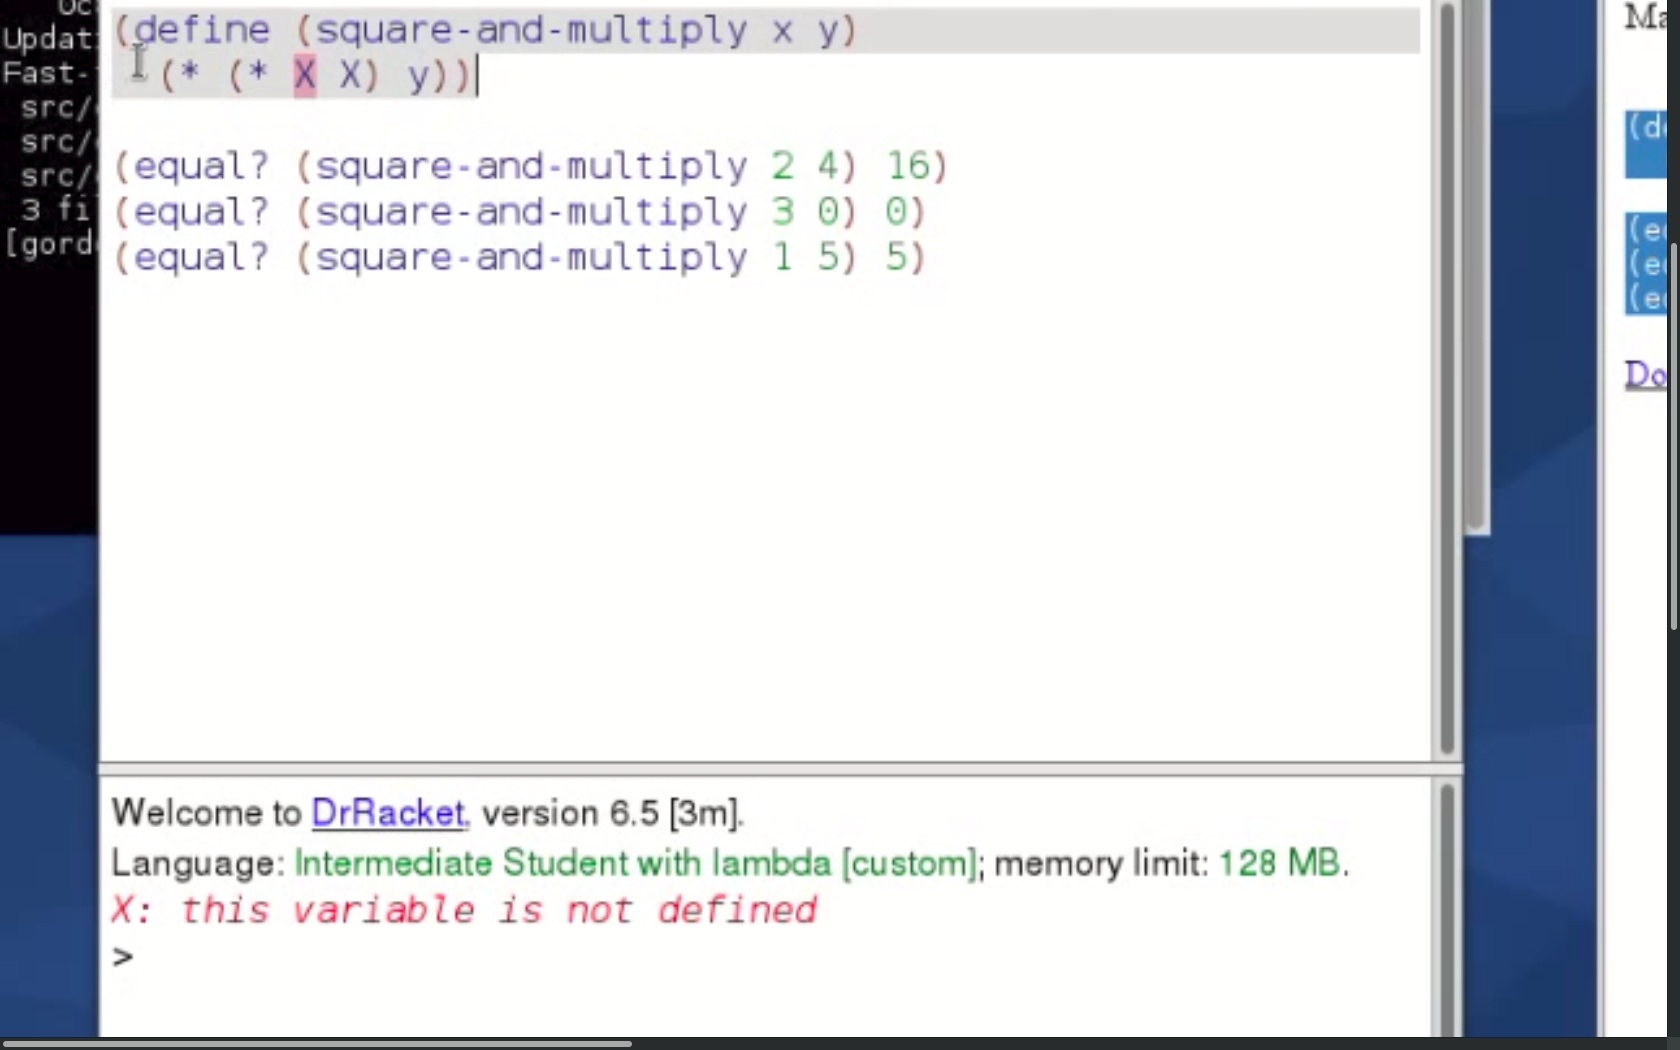
\includegraphics[scale=.17]{R2Rshot}
\end{frame}

\begin{frame}
  \frametitle{Clojure Standard Error Messaging}
\end{frame}

\begin{frame}
  \frametitle{Clojure Modified Error Messaging}
\end{frame}




\section{Work in progress}

\begin{frame}
  \frametitle{Work in progress}
\begin{itemize}
\item Continued usability study 
\item Project re-structuring
\end{itemize}
\end{frame}

%%% If you are including verbatim text, make the frame fragile
\begin{frame}[fragile]
\frametitle{Including text verbatim}
Typically you include program code verbatim:
\begin{verbatim}
(defn get-match-name [fname]
  "extract a function name from a qualified name"
  (let [m (nth (re-matches #"(.*)\$(.*)" fname) 2)
        matched (if m m (nth (re-matches #"(.*)/(.*)" 
            fname) 2))]
    (if matched
      (check-if-anonymous-function 
           (lookup-funct-name matched))
      fname)))
\end{verbatim}
\end{frame}

\end{document}

